\documentclass[11pt]{article}
\usepackage{latexsym}
\usepackage{amsmath}
\usepackage{amssymb}
\usepackage{amsthm}
\usepackage{epsfig}
% \usepackage{graphics}
\usepackage[tight]{subfigure}

\usepackage{amsmath}

\usepackage{bm}
\usepackage{graphicx}
\usepackage{caption}
\usepackage{subcaption}
\usepackage{float}

\DeclareMathOperator*{\argmax}{arg\,max}
\DeclareMathOperator*{\argmin}{arg\,min}
\DeclareMathOperator*{\minimize}{min}
\DeclareMathOperator*{\maximize}{max}

\usepackage{algorithm}
 %on linux you may need to run sudo apt-get install texlive-full to install algorithm.sys
\usepackage{algorithmic}

\usepackage{verbatim}

\newcommand{\handout}[5]{
  \noindent
  \begin{center}
  \framebox{
    \vbox{
      \hbox to 5.78in { {#1} \hfill #2 }
      \vspace{4mm}
      \hbox to 5.78in { {\Large \hfill #5  \hfill} }
      \vspace{2mm}
      \hbox to 5.78in { {\em #3 \hfill #4} }
    }
  }
  \end{center}
  \vspace*{4mm}
}

\newcommand{\lecture}[5]{\handout{#1}{#2}{#3}{#4}{#5}}
\newcommand{\collision}[0]{\mathrm{collision}}
\newcommand{\nocollision}[0]{\overline{\collision}}

\newcommand*{\QED}{\hfill\ensuremath{\square}}

\newtheorem{theorem}{Theorem}
\newtheorem{corollary}[theorem]{Corollary}
\newtheorem{lemma}[theorem]{Lemma}
\newtheorem{observation}[theorem]{Observation}
\newtheorem{proposition}[theorem]{Proposition}
\newtheorem{definition}[theorem]{Definition}
\newtheorem{claim}[theorem]{Claim}
\newtheorem{fact}[theorem]{Fact}
\newtheorem{assumption}[theorem]{Assumption}
\newtheorem{note}[theorem]{Note}

% 1-inch margins, from fullpage.sty by H.Partl, Version 2, Dec. 15, 1988.
\topmargin 0pt
\advance \topmargin by -\headheight
\advance \topmargin by -\headsep
\textheight 8.9in
\oddsidemargin 0pt
\evensidemargin \oddsidemargin
\marginparwidth 0.5in
\textwidth 6.5in

\parindent 0in
\parskip 1.5ex
%\renewcommand{\baselinestretch}{1.25}

\begin{document}

\lecture{Statistical Techniques in Robotics (16-831, S22)}{Lecture \#22
  (Monday, April 11)}{Lecturer: Kris Kitani}{Scribes: Xuanbai Chen, Tzu-Hsuan Yang (Group 1)}{Imitation Learning}

\section{Review}
In the last lecture, we continue talking about the RL approaches. At this time, we mainly focused on the Policy-based approaches which will be mainly included in Section~\ref{PGM} and the Actor-Critic method, which is the hybrid of Policy-based and Value-based methods, in Section~\ref{ACM}

\subsection{Policy Gradient Methods}
\label{PGM}
By leveraging the gradient ascent, we can update the parameters to obtain the best policy that maximizes the expected return. The objective of policy gradient method is listed below:
\begin{align}
    \hat{\theta} & = \argmax_{\theta} \mathbb{E}_{p_\theta(\zeta)}\left[\sum_{t=0}^Tr^{(t)}\right] \\
    & = \argmax_{\theta} J(\theta)
\end{align}
By changing the linear approximation of the objective function with quadratic regularization and solving for the parameter that optimizes the Lagrangian, we can make the optimization process as follows:
\begin{align*}
    & \nabla_\theta\{\alpha(J(\theta^{'})+\langle\theta-\theta^{'}, \nabla_\theta^{'}J(\theta^{'})\rangle - \frac{1}{2}||\theta-\theta^{'}||^2)\} = 0 \\
    \Rightarrow & \;\theta \leftarrow \theta^{'} + \alpha \nabla_{\theta^{'}}J(\theta^{'})
\end{align*}
From the definition of $\nabla_\theta J(\theta)$, we can derive that it equals to:
\begin{align*}
    \nabla_\theta J(\theta) = \frac{1}{N}\sum_{n=1}^N \Bigg( \sum_{t=1}^T \nabla_\theta \ln \pi_\theta(a^{(n, t)}|s^{(n, t)}) \Bigg) \Bigg( \sum_{t=1}^T r^{(n, t)} \Bigg)
\end{align*}

\subsubsection{Monte-Carlo Policy Gradient}
By plugging the equation above to the Monte-Carlo algorithm, we can acquire the algorithm of Monte-Carlo policy gradient below.
\begin{algorithm}[H]
\caption{MC-Policy-Gradient($\pi_\theta,a$)}
\begin{algorithmic}[1]
\FOR{$e=1,\;\cdots,\;E$}
\STATE $\{s^{(t)}, a^{(t)}, r^{(t)}\}_{t=0}^T \sim \mathcal{E}|\pi_\theta$
\STATE $G^{(0)} = \sum_{t=0}^T r^{(t)}$ 
\FOR{$t=0,\;\cdots,\;T$}
\STATE $\theta \leftarrow \theta + \alpha \Big( \nabla_\theta \log \pi_\theta (a^{(t)}|s^{(t)}) \Big) \Big( G^{(0)} \Big) $
\ENDFOR
\ENDFOR
\RETURN $\pi_\theta$
\end{algorithmic}
\end{algorithm}

However, there exists a big problem which the variance of the algorithm is high. Two methods can ease the problem, which the former is to enforce causality and the latter to remove gradient bias with a baseline offset.
%
The principle enforcing causality is to depend only on future reward at time $t$.
\begin{align*}
    \nabla_\theta J(\theta) \approx \frac{1}{N}\sum_{n=1}^N \Bigg( \sum_{t=0}^T \nabla_\theta \ln \pi_\theta(a^{(n, t)}|s^{(n, t)}) \Bigg) \Bigg( \sum_{t^{'}=t}^T r^{(n, t^{'})} \Bigg)
\end{align*}

By adjusting the gradient By subtracting some offset b, we can adjust the gradient and reduce the problem of large gradient variance,
\begin{align*}
    \nabla_\theta J(\theta)= \int_\theta p_\theta(\zeta) \nabla_\theta \ln p_\theta(\theta)r(\zeta)d\zeta
\end{align*}

\subsubsection{Policy Gradient}
By using these two strategies and putting them together, we can obtain the policy gradient algorithm as follows:
\begin{algorithm}[H]
\caption{Policy Gradient($\pi_\theta, \alpha, b$)}
\begin{algorithmic}[1]
\FOR{$e=1,\;\cdots,\;E$}
\STATE $\{s^{(t)}, a^{(t)}, r^{(t)}\}_{t=0}^T \sim \mathcal{E}|\pi_\theta$
\FOR{$t=0,\;\cdots,\;T$}
\STATE $G^{(t)} = \sum_{i=t}^T r^{(i)}$  \hfill (1) Enforce causality
\STATE $\theta \leftarrow \theta + \alpha [G^{(t)}-b] \nabla_\theta \log \pi_\theta (a^{(t)}|s^{(t)}) $ \hfill (2) Subtract baseline
\ENDFOR
\ENDFOR
\RETURN $\pi_\theta$
\end{algorithmic}
\end{algorithm}
In conclusion, the positives of the policy gradient are as follows: (1) Doesn't require model and learns from interaction. (2) Effective for high-dimensional or continuous action spaces (all methods so far assumed finite action space). (3) Can encode prior knowledge when designing policy architecture. (4) Finds the optimal stochastic policy and naturally explores due to stochasticity.
%
While the negatives of the policy gradient are as follows: (1) Gradient is typically high variance and leads to slow convergence. (2) Small step size leads to slow convergence (3) Typically converge to local minima instead of global minima. (4) Exploding or zero gradient.

\subsection{Actor Critic}
\label{ACM}

In the policy gradient algorithm, we need to acquire $\sum_{t=1}^T r^{(t)}$ to compute the gradient. Actor Critic methods can use the model-free prediction for the return value estimator. The equation are as below:
$$\nabla_\theta J(\theta) = \mathbb{E}_{p_\theta} [(\sum_{t=1}^T \nabla_\theta \ln \pi_\theta (a^{(t)} | s^{(t)}) (G_\phi^{(t)}) ]$$
where $G_\phi$ is function approximation of the return value parameterize by $\phi$. After removing the gradient bias of policy gradient, we can get the advantage function.
$$A(a^{(t)}, s^{(t)}) = Q_\phi (a^{(t)}, s^{(t)}) - V_\psi (s^{(t)})$$
So the policy gradient with advantage function is as follow:
$$\nabla_\theta J(\theta) = \mathbb{E}_{p_\theta} [(\sum_{t=1}^T \nabla_\theta \ln \pi_\theta (a^{(t)} | s^{(t)}))(\sum_{i=t}^T A_\phi (a, s))]$$

The Advantage-MC-Actor-Critic algorithm and Advantage-TD-Actor-Critic algorithm are as below:
\begin{algorithm}[H]
\caption{Advantage-MC-Actor-Critic(\pi_{\epsilon}, Q_\phi, V_\psi, \alpha, \beta, \kappa)}
\label{algo:qmc-ac}
\begin{algorithmic}[1]
\FOR{$e=0,\;\cdots,\;E$}
\STATE $\{ s^{(t)}, a^{(t)}, r^{(t)} \}_{t=0}^T$ \sim $\mathcal{\epsilon} | \pi_{\epsilon}$ 
\FOR{$t=0,\;\cdots,\;T$}
\STATE $G^{(t)} \leftarrow \sum_{t=1}^T r^{(i)}$ \hfill MC estimate
\STATE $\psi \leftarrow \psi + \kappa[G^{(t)} - V_\psi (s^{(t)})] \nabla_\psi V_\psi(s^{(t)})]$ \hfill V update
\STATE $\phi \leftarrow \phi + \beta[G^{(t)} - Q_\phi (a^{(t)}, s^{(t)})]\nabla Q_\phi (a^{(t)}, s^{(t)})$ \hfill Q update
\STATE $\theta \leftarrow \theta + \alpha \nabla \log \pi_\theta (a^{(t)} | s^{(t)}) \dot Q_\phi (a^{(t)}, s^{(t)})$ \hfill Policy update

\ENDFOR
\ENDFOR
\end{algorithmic}
\end{algorithm}
\begin{algorithm}[H]
\caption{Advantage-TD-Actor-Critic(\pi_{\epsilon}, Q_\phi, V_\psi, \alpha, \beta, \kappa)}
\label{algo:qtd-ac}
\begin{algorithmic}[1]
\FOR{$e=0,\;\cdots,\;E$}
\STATE $\{ s^{(t)}, a^{(t)}, r^{(t)} \}_{t=0}^T \sim \mathcal{\epsilon} | \pi_{\epsilon}$ 
\FOR{$t=0,\;\cdots,\;T$}
\STATE $\delta_V \leftarrow r^{(t)} + V_\psi (s^{(t+1)})$ \hfill TD V estimate
\STATE $\psi \leftarrow \psi + \kappa[\delta_V - V_\psi (s^{(t)})] \nabla_\psi V_\psi(s^{(t)})]$ \hfill V update
\STATE $\delta_Q \leftarrow r^{(t)} + Q_\phi (a^{t+1}, s^{(t+1)})$ \hfill TD Q estimate
\STATE $\phi \leftarrow \phi + \beta[\delta_Q - Q_\phi (a^{(t)}, s^{(t)})]\nabla Q_\phi (a^{(t)}, s^{(t)})$ \hfill Q update
\STATE $\theta \leftarrow \theta + \alpha \nabla \log \pi_\theta (a^{(t)} | s^{(t)}) \dot Q_\phi (a^{(t)}, s^{(t)})$ \hfill Policy update

\ENDFOR
\ENDFOR
\end{algorithmic}
\end{algorithm}














\newpage

\section{Summary}
\subsection{Imitation Learning}
\subsubsection{Motivation for Imitation Learning}
\normalfont
As what we have learned before, the training process of the reinforcement learning algorithm is that the model learns on its own by a combination of exploration and exploitation of its environment and tries to maximize a scalar reward to get the policy. However, this training process can take a very long time to lean a policy because it has to learn everything from experience. To think of a better (faster) way to learn, we then have the Imitation Learning also known as Learning from Demonstration, apprenticeship learning, behaviour cloning, inverse reinforcement learning. Just as the algorithm name, the Imitation Learning (IL) learns a policy from demonstrated expert behaviour. In addition, sometimes the reward function defined in the reinforcement learning is too complex to define, it is easier to just show examples as what have be given in the IL. There are three types of IL algorithm, including Passive IL, Active IL, and Interactive IL, which will be discussed into detail later.
\subsubsection{Definition for Imitation Learning}
\normalfont
The Imitation Learning can be formally defined as : 
\begin{align}
    \mathcal{A}_{\mathrm{IL}}:\left\langle\mathcal{D}^{*}, \pi^{*}, \mathcal{T}, \mathcal{R}\right\rangle \rightarrow \pi
\end{align}
And this formula includes the following parts
\subparagraph{Expert Demonstrations}
\begin{align}
    \mathcal{D}^{*}=\left\{\boldsymbol{\zeta}_{n}\right\}_{n=1}^{N} \sim \mathcal{E} \mid \pi^{*}
\end{align}
\normalfont

Expert demonstrations are trajectories, denoted as $\zeta_{n}$, sampled from the optimal policy $\pi^{*}$, which is used by IL algorithm to learn a good policy. These trajectories are a sequence of variables such as a sequence of states and actions. 
\begin{align}
    \zeta=\left\{s^{(0)}, s^{(1)}, \ldots, s^{(T)}\right\}\label{eq:state sequence} \\
 \zeta=\left\{s^{(0)}, a^{(0)}, s^{(1)}, \ldots, a^{(T-1)}, s^{(T)}\right\}\label{eq:action sequence}
\end{align}
Eq.(\ref{eq:state sequence}) shows the expert demonstrations in state sequence and Eq.(\ref{eq:action sequence}) gives the state-action pair sequence in expert demonstrations. We also discussed in the lecture that we can have other different forms for expert demonstrations depends on specific algorithms.
\subparagraph{Optimal Policy (Oracle)}
\begin{align}
    a \sim \pi^{*}(s)
\end{align}
The optimal policy also called oracle is where expert demonstrations are sampled. In the IL algorithm, this is not always accessible during the training process. The optimal policy is only available for interactive IL, which is,  during the learning, we do not get the entire policy, but we can get samples from it (as the equation shows). For example, during the learning, the algorithm can query the optimal policy at every time step, and this interactive oracle feedback would tell you what action you should but not gives you the full parametric form. 
\subparagraph{Dynamics Function}
\begin{align}
    \mathcal{T} = P\left(s^{\prime} \mid s, a\right)
\end{align}
Dynamic Function shows the probability that an action a in the state s leads to state $s^{\prime}$ and . In the IL algorithm, this is also not always accessible during the training process. Only active IL and interactive IL can optionally take this into training progress. 
\subparagraph{Reward Function}
\begin{align}
    \mathcal{R} = P\left(s, a, s^{\prime}\right)
\end{align}
Similar as the Reinforcement Learning, the reward function in imitation learning is also defined as what the agent achieves at a particular state $s$, taking action $a$ and reaches next state $s'$. In the next section, we can find that the reward function of some algorithms can be sampled from the environment, while the others can't.


\subsection{3 Types of Imitation Learning}
\normalfont
As we discussed in the previous section, based on what information the model could access to, we can divide the IL algorithm into three categories. 
\begin{table}[h]
    \centering
    \begin{tabular}{|c|c|c|c|}
        \hline& Passive IL &  Active IL & Interactive IL\\
        \hline Demonstrations $\mathcal{D}$ & yes & yes & optional \\ 
        \hline Environment $\mathcal{E}$ & no & yes & yes \\
        \hline Oracle $\pi$ & no & no & yes \\
        \hline Dynamics $\mathcal{T}$ & no & optional & optional \\
        \hline Reward $\mathcal{R}$ & no & optional & optional \\
        \hline
    \end{tabular}
    \caption{3 Types of Imitation Learning}
    \label{tab:my_label}
\end{table}

\subsubsection{Passive Imitation Learning}
\normalfont
Passive Imitation Learning also known as supervised learning, behaviour cloning only have access to demonstrations. Passive IL involves learning a policy that performs nearly as well as an expert’s policy based on a set of trajectories of that policy. However, if the agent visits the state that the expert trajectories never learns, the agent doesn't know what to do at this state and may cause error. With many unseen states in out test distribution, the accumulation of small errors will lead to Covariate Shift. In other words, the Passive IL works well if the problem is not difficult and having expert demonstrations responds to all possible states then the model knows how to behaviour when encountering every possible state. Generally speaking, the Passive IL can only models short-term (one-shot) behaviour and cannot model long-term behaviour well. 

Taking that learning how to play Golf as an analogy. The objective policy function is to being experts in this sport and know how to play. For passive learning, people don't have any access to the real golf court. They are only given a book contained with the instructions of how to play golf (seems like the expert demonstrations). Based on these expert demonstrations, they have to consider how to play golf in the final testing process.

\begin{figure}[h]
\centering
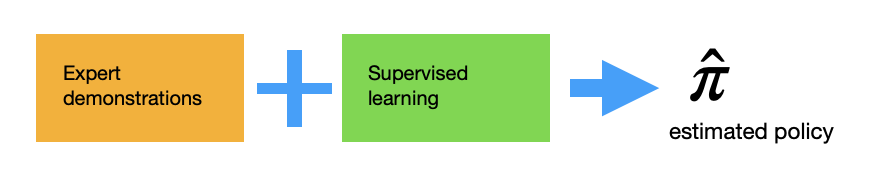
\includegraphics[width=0.5\textwidth]{Passive.png}
\caption{Passive Imitation Learning Paradigm}
\end{figure}

\subsubsection{Active Imitation Learning}
In the Passive IL we knows that if we have the full expert trajectories, our models can learn well. However, generating such trajectories is often tedious or even impractical for an expert (e.g., real-time low-level control of multiple game agents). In order to address this issue, active Imitation Learning have accessed to expert demonstrations and environments and can optionally access the dynamics and rewards. In other words, the model can learn policy from expert demonstrations and have opportunities to implement those learned policy in the environment and to improve it. However, sometimes just mimicking expert demonstrations is not helpful because we can't generalize to new environments. In this scenario, understanding why (reward function) we take an action help us to generalize our learning better. And this lead to Inverse Reinforcement Learning, a type of Active IL, which will be discussed in the later section.

Similar as passive imitation learning, people are still given a book contained the instructions of how to play golf in active imitation learning. However, in this time, they have the chance to enter the golf court for practising. They can experience what the real environment is like and conduct lots of experiments in it based on the instruction book (expert demonstrations).
\begin{figure}[h]
\centering
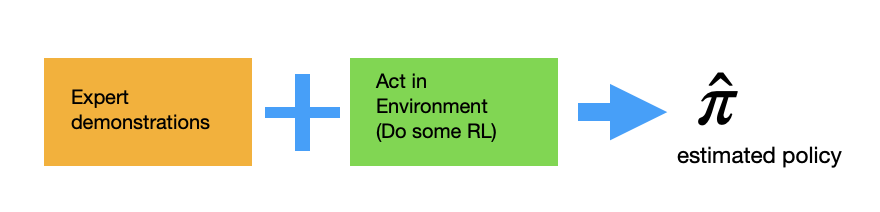
\includegraphics[width=0.5\textwidth]{Active.png}
\caption{Active Imitation Learning Paradigm}
\end{figure}

\subsubsection{Interactive Imitation Learning}
Interactive Imitation Learning accesses the expert demonstrations optionally. Instead, it accesses the optimal policy (oracle) during the learning process. This iterative algorithm assumes that we have accessed to an interactive demonstrator at the same time during the training, who we can query. This involves learning some demonstrations from the expert, and applying supervised learning to learn a policy.Then rolling out this policy in the environment, and querying the expert to evaluate the roll-out trajectory. In this way, we get more training data, which we feedback to supervised learning.

As for the interactive imitation learning algorithm, people can also act in the environment to do exercises for playing the golf. However, instead of only obtaining the original static instructions, they can get interactive feedback this time. To be specific, it seems like there exists a teacher helping you on the skills of playing golf. He can provide a unique instruction for you. If you perform poor in swinging, they can design corresponding exercise for you to improve the swinging skills.

One simple concern is that since we have already had access to the environment and the expert demonstrations, why can't we just get all demonstrations and the optimal policy? The reason is that we only get access to samples of the optimal policy and demonstrations. In this way, we have no access to the whole optimal policy.

\begin{figure}[h]
\centering
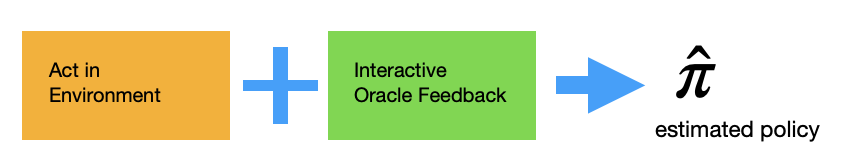
\includegraphics[width=0.5\textwidth]{Interactive.png}
\caption{Interactive Imitation Learning Paradigm}
\end{figure} 

\subsection{Inverse Reinforcement Learning(IRL)}
\subsubsection{Motivation for Inverse Reinforcement Learning}
\normalfont
Inverse Reinforcement Learning is a type of active IL, involves learning an expert’s objectives, values, or rewards with the aid of using insights of its behavior. In this algorithm, the model not only learns an estimated optimal policy but also attempt to learn an reward function. 

\subsubsection{IRL vs RL}
Model-based Reinforcement Learning learns the optimal policy by the dynamics model and reward function. However, sometimes the reward function can be really hard to define. Therefore, in IRL, We learn the reward function from the expert demonstrations and feed this reward function into the RL training process to get the optimal policy. The advantage of using IRL is that the expert demonstrations can be transferred to new (but similar) environments, not just mimicry. The output of IRL is a reward function. 

In this setting, the Inverse reinforcement learning is crucial since some reinforcement learning algorithm does not show good generalization ability when leveraging in a new environment. The reason is that sometimes some RL algorithms just simply mimic the experts demonstrations, they have no idea about the principle of the whole environment. In this way, understanding why (reward function) we take an action can help us to generalize our learning better.

\begin{figure}[h]
\centering
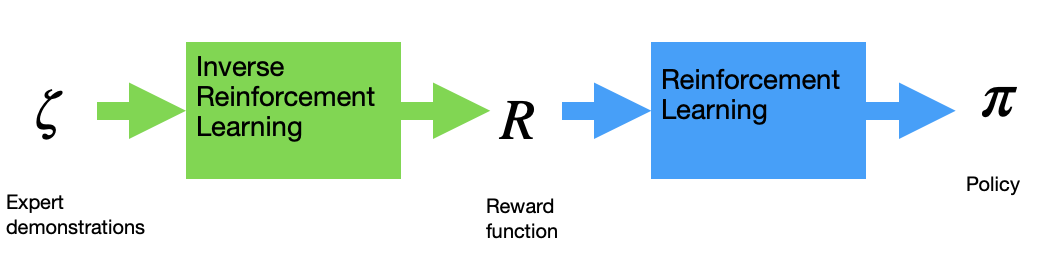
\includegraphics[width=0.5\textwidth]{IRL.png}
\caption{Inverse Reinforcement Learning Paradigm}
\end{figure}


\subsubsection{5 Types of IRL Algorithm}

\subsubsection{Linear Program IRL}
Introduced in~\cite{ng2000algorithms}, the linear function approximation in large state spaces is defined as follows:
\begin{align}
    \hat{\boldsymbol{\theta}}=\underset{\boldsymbol{\theta}}{\arg \max }\left\{\sum_{n} \hat{V}^{\pi^{*}}\left(s_{0}\right)-\hat{V}^{\pi_{n}}\left(s_{0}\right)\right\} \\
s.t. \left|\theta_{d}\right| \leq 1 \quad \forall d
\end{align}


\subsubsection{Matrix Game IRL}
The method~\cite{syed2007game} is based on a game-theoretic view of the problem, which leads naturally to a direct application of the multiplicative-weights algorithm for playing repeated matrix games. The equation is defined as follow:
\begin{align}
    \min _{\theta}\left\{\max _{\pi} \theta \cdot \mu(\pi)-\theta \cdot \mu\left(\pi_{E}\right)\right\}
\end{align}

\subsubsection{Max Margin IRL}
They set an assumption that the expert tries to maximize a reward function that is expressible as a linear combination of known features, and gives an algorithm for learning the task demonstrated by the expert. Abbeel \emph{et al.}~\cite{abbeel2004apprenticeship} design the method that is based on using “inverse reinforcement learning” to try to recover the unknown reward function.
\begin{align}
    \begin{array}{ll}\min _{\theta} & \lambda\|\theta\|_{2}+\sum_{i} \xi_{i} \\ \text { s.t. } & \theta^{\top}\left(\mu\left(\pi^{*}\right)-\mu\left(\pi_{i}\right)\right) \geq\left(1-\xi_{i}\right) \quad \forall i\end{array}
\end{align}

\subsubsection{Structured Output Max Margin IRL}
Ratlif \emph{et al.}~\cite{ratliff2006maximum} frame learning imitation learning of sequential, goal-directed behavior as a maximum margin structured prediction problem over a space of policies.
\begin{align}
    \min _{\theta} \frac{1}{2}\|\theta\|_{2}^{2}+\frac{\lambda}{D} \sum_{d} \beta_{d}\left\{\max _{\eta}\left(\theta^{\top} F_{d}+l_{d}^{\top}\right) \eta-\theta^{\top} F_{d} \eta_{d}\right\}
\end{align}



\subsubsection{Maximum Entropy IRL}
\cite{ziebart2008maximum} introduces a probabilistic approach based on the principle of maximum entropy by providing a well-defined, globally normalized distribution over decision sequences.
\begin{align}
   \min _{\theta} & \sum_{\zeta} p(\zeta ; \theta) \log p(\zeta ; \theta) \\ & \text { s.t. } \sum_{\zeta} p(\zeta ; \theta) \mu(\zeta)=\sum_{d} p_{u}\left(\zeta_{d}\right) \mu\left(\zeta_{d}\right) 
\end{align}
% Now, we introduce the Randomized Weighted majority Algorithm (RWMA), listed as Algorithm \ref{algo:rwma} below. It is known by many different names, such as Exponentiated Weighted Majority, Hedge Algorithm etc. The key difference from WMA is that we create a multinomial distribution using the weights and make the learner prediction via sampling from this distribution (Line 5, 6).

% \begin{algorithm}[H]
% \caption{Randomized Weighted Majority Algorithm (RWMA)}
% \label{algo:rwma}
% \begin{algorithmic}[1]
% \STATE $\textbf{w}^{(1)} \leftarrow \{w_n^{(1)}=1\}_{n=1}^N$ \hfill $\triangleright$ Weight initialization
% \STATE $\eta\leq\frac{1}{2}$\hfill $\triangleright$ Penalty rate initialization
% \FOR{$t=1,\;\cdots,\;T$}
% \STATE \textsc{Receive} ($\textbf{x}^{(t)}\in\{-1, 1\}^N$) \hfill $\triangleright$ Receive experts predictions
% \STATE $I\sim$ \textsc{Multinomial}($\textbf{w}^{(t)}/\Phi^{(t)}$), where $\Phi^{(t)}=\sum_{n=1}^Nw_n^{(t)}$
% \STATE $\hat{y}^{(t)}=h_i(\textbf{x}^{(t)})$ \hfill $\triangleright$ Make learner prediction via sampling
% \STATE \textsc{Receive} ($y^{(t)}\in\{-1, 1\}$) \hfill $\triangleright$ Receive actual answer
% \STATE $w_n^{(t+1)}\leftarrow w_n^{(t)}\big(1-\eta\cdot\textbf{1}[y^{(t)}\neq h_n(\textbf{x})^{(t)}]\big)$ \hfill $\triangleright$ Weight update
% \ENDFOR
% \end{algorithmic}
% \end{algorithm}

% Now, let's derive the mistake bound for RWMA. We will find that the expected number of mistakes for RWMA is upper bounded and the mistake bound is better than a factor of 2, when compared to the WMA. But first, we state a simple lemma to help derive further results in Theorem 9.


% \lemma{$e^x\geq 1+ x$ for all $x\in\mathbb{R}$.}\label{lemma:2}
% \proof{One can easily show the above inequality by applying Taylor expansion to $e^x$.}
% \theorem{(Mistake bound of RWMA) Let $M^{(t)}, m_i^{(t)}$ respectively be the number of mistakes that have been made by the RWMA learner and the $i$-th hypothesis until the time step $t$, and $N, \eta$ be the number of experts and the penalty rate. Then, expected mistakes of learner $\mathbb{E}[M^{(t)}]$ is upper-bounded as:
% $$\mathbb{E}[M^{(t)}]\leq (1+\eta)m_i^{(t)} + \frac{\log{N}}{\eta}$$}\label{theorm:rwma}
% \proof{Lets again define the potential function $\Phi^{(t)}$ for RWMA as the sum of weights:
% \begin{align}
%   \Phi^{(t)} = \sum_{n=1}^N w_n^{(t)}\label{eq:rwma_potential}
% \end{align}
% By the weight update rule of RWMA, $w_n^{(t+1)}$ can be analytically calculated from $w_n^{(t)}$ as follows:
% \begin{align}
%     w_n^{(t+1)}= \big(1-\eta\cdot\textbf{1}[y^{(t)}\neq y_n^{(t)}]\big)w_n^{(t)}=\big(1-\eta\alpha_n^{(t)}\big)w_n^{(t)}\;\;\;\;\;(\text{where} \;\alpha_n^{(t)}=\textbf{1}[y^{(t)})\neq y_n^{(t)}]\label{eq:rwma_weight}
% \end{align}
% By combining Eq. (\ref{eq:rwma_weight}) \& (\ref{eq:rwma_potential}), one can derive the mathematical relation between $\Phi^{(t+1)}$ and $\Phi^{(t)}$ as follows:
% \begin{align}
%     \Phi^{(t+1)}=\sum_n w_n^{(t+1)}&=\sum_n (1-\eta\alpha_n^{(t)})w_n^{(t)}\;\;\;(\because \text{Eq.}\; (\ref{eq:rwma_weight}))\nonumber\\
%     &=\sum_n w_n^{(t)} - \sum_n \eta\alpha_n^{(t)}w_n^{(t)}\nonumber\\
%     &=\Phi^{(t)} - \frac{\Phi^{(t)}}{\Phi^{(t)}}\sum_n \eta\alpha_n^{(t)}w_n^{(t)}\nonumber\\
%     &=\Phi^{(t)} - \Phi^{(t)}\eta\sum_n \alpha_n^{(t)}\frac{w_n^{(t)}}{\Phi^{(t)}}\nonumber\\
%     &=\Phi^{(t)} - \Phi^{(t)}\eta\sum_n \alpha_n^{(t)}p_n^{(t)}\;\;\;(\text{where}\;p_n^{(t)}=\frac{w_n^{(t)}}{\Phi^{(t)}})\nonumber\\
%     &=\Phi^{(t)}\Big(1-\eta\sum_n\alpha_n^{(t)}p_n^{(t)}\Big)\label{eq:rwma_abc}
% \end{align}
% Assuming all weights are initialized to 1, $\Phi^{(T+1)}$ can be calculated by recursively applying Eq. ({\ref{eq:rwma_abc}}) as follows:
% \begin{align}
%     \Phi^{(T+1)}=\Phi^{(1)}\prod_{t=1}^{T}\Big(1-\eta\sum_n\alpha_n^{(t)}p_n^{(t)}\Big)=N\prod_{t=1}^{T}\Big(1-\eta\sum_n\alpha_n^{(t)}p_n^{(t)}\Big)\label{eq:rwma_xyz}
% \end{align}
% We can now derive the upper bound of $\Phi^{(T+1)}$ by combining Lemma \ref{lemma:2} and Eq. (\ref{eq:rwma_xyz}) as follows:
% \begin{align}
%     \Phi^{(T+1)}&=N\prod_{t=1}^{T}\Big(1-\eta\sum_n\alpha_n^{(t)}p_n^{(t)}\Big)\nonumber\\
%     &\leq N\prod_{t=1}^T\exp{\Big(-\eta\sum_n\alpha_n^{(t)}p_n^{(t)}\Big)}\;\;\;(\because \text{Lemma}\;\ref{lemma:2})\nonumber\\
%     &=N\exp{\Big(-\eta\sum_{t=1}^{T}\mathbb{E}\big[\textbf{1}[y^{(t)}\neq\hat{y}^{(t)}]\big]\Big)}\;\;\;(\because\;\sum_n\alpha_n^{(t)}p_n^{(t)}=\mathbb{E}_p\big[\textbf{1}[y^{(t)}\neq\hat{y}^{(t)}]\big])\nonumber\\
%     &=N\exp{\big(-\mathbb{E}[M^{(T)}]\big)}\;\;\;(\because\;\text{definition of}\;M^{(t)})\label{eq:rwma_upper}
% \end{align}
% By applying the same argument as in WMA, the lower bound of $\Phi^{(T+1)}$ is $(1-\eta)^{m_n^{(T)}}$.
% \begin{align}
%     \Phi^{(T+1)}\geq(1-\eta)^{m_n^{(T)}}\label{eq:rwma_lower}
% \end{align}
% By combining Eq. (\ref{eq:rwma_upper}) \& (\ref{eq:rwma_lower}), we can now derive the mathematical relation between $\mathbb{E}[M^{(t)}]$ and $m_n^{(t)}$ as follows:
% \begin{align}
%     (1-\eta)^{m_n^{(T)}}\leq \Phi^{(T+1)} \leq N\exp{\big(-\mathbb{E}[M^{(T)}]\big)}\label{eq:rwma_init}
% \end{align}
% Finally, we can compute the (upper) bound of expected mistakes $\mathbb{E}[M^{(t)}]$ by combining the bounds of $\Phi^{(t+1)}$ (Eq. (\ref{eq:rwma_init})) and Lemma \ref{lemma:1} as follows:
% \begin{align*}
%     m_n^{(T)}\log(1-\eta) &\leq \log N - \eta\mathbb{E}[M^{(T)}]\\
%     m_n^{(T)}(-\eta-\eta^2)&\leq \log N - \eta\mathbb{E}[M^{(T)}] \;\;\;(\because\; \text{Lemma}\;\ref{lemma:1})\\
%     -m_n^{(T)}(1+\eta)&\leq\frac{\log N}{\eta} - \mathbb{E}[M^{(T)}]\\
%     \mathbb{E}[M^{(T)}]&\leq (1+\eta)m_n^{(T)} + \frac{\log N}{\eta}
% \end{align*}
% Therefore, we have obtained the upper bound of expected regret for RWMA.\QED
% }

% We are now interested in the performance (regret bound) of RWMA algorithm.
% \theorem{RWMA is a no-regret algorithm.}
% \proof{By the definition of regret and Theorem \ref{theorm:rwma}}, we could obtain the upper bound of \textit{expected regret} of RWMA, $\mathbb{E}[R]$, as follows:
% \begin{align}
%     \mathbb{E}[R] = \mathbb{E}[M^{(T)}] - m_n^{(T)} \leq \eta m_n^{(T)} + \frac{\log N}{\eta} \label{eq:rwma_final}
% \end{align}
% If we set $\eta$ to $\frac{1}{\sqrt{T}}$, both $\eta m_n^{(T)}$ and $\frac{\log N}{\eta}$ follow $O(\sqrt{T})$.\\
% Thus, $\frac{\mathbb{E}[R]}{T} = \Big(\eta m_n^{(T)} + \frac{\log N}{\eta}\Big) \propto \frac{1}{\sqrt{T}}\rightarrow 0\;\text{as}\;T\rightarrow\infty$.\QED

{
\bibliography{refs}
\bibliographystyle{abbrv}
}

\newpage
\section{Appendix}

In this section, we would like to introduce some foundational methods for IRL, which can mainly be divided into four classes: margin based optimization, entropy based optimization, Bayesian inference, classification, and regression. In this scribe note, we mainly introduce the first two types of methods.

\subsection{Margin Optimization}
Maximum margin prediction aims to learn a reward function that explains
the demonstrated policy better than alternative policies by a margin. The
methods under this category aim to address IRL’s solution ambiguity by converging on a solution that maximizes some margin. We broadly organize the methods that engage in margin optimization based on the type of the margin that is used.

\subsubsection{Margin of optimal from other actions or policies}
One of the earliest and simplest margins chosen for optimization is the sum of differences between the expected value of the optimal action and that of the next-best action over all states,
$$ \sum_{s \in S} Q^{\pi} (s, a^*) - \max_{a \in A | {a^*}} Q^{\pi} (s, a)$$
where $a^*$ is the optimal action for s.

An early and foundational method that optimized the margin given in equation above is [A. Ng, S. Russell, Algorithms for inverse reinforcement learning], which takes in the expert’s policy as input. It formulates
a linear program to retrieve the reward function that not only produces the given policy as optimal output from the complete MDP, but also maximizes the margin shown above. In addition to maximizing this margin, it also prefers reward functions with smaller values as a form of regularization.

\subsubsection{Margin of observed from learned feature expectations}
Adoption of the feature-based reward function led to several methods optimizing margins that utilized feature expectations. Some of these methods seek a reward function that minimizes the margin between the feature expectations of a policy computed by the learner and the empirically computed feature expectations from the expert’s trajectory.
$$|\mu^{\phi}(\pi) - \hat{\mu}^{\phi} (D)|$$
We refer to this margin as the feature expectation loss.

Two foundational methods [P. Abbeel, A. Y. Ng, Apprenticeship learning via inverse reinforcement learning] that maximize the feature expectation loss
margin of the equation above are max-margin and projection. Noting that the learner does not typically have access to the expert’s policy, both these methods take a demonstration as input. The methods represent the reward function as a linear, weighted sum of feature functions.

\subsubsection{Observed and learned policy distributions over actions}
An alternative to minimizing the feature expectation loss is to minimize the probability difference between stochastic policies
$$\hat{\pi}_{E} (a \mid s) - \pi_{E} (a \mid s)$$
for each state. As the behavior of expert is available instead of its policy, the difference above is computed using the empirically estimated state visitation frequencies and the frequencies of taking specific actions in the states. HYBRID-IRL [G. Neu, C. Szepesv´ari, Apprenticeship Learning using Inverse Reinforcement Learning and Gradient Methods] uses the equation above in the margin optimization problem, solving the optimization using gradient descent in the space of reward hypotheses.

\subsection{Entropy Optimization}
IRL is essentially an ill-posed problem because multiple reward functions can explain the expert’s behavior. The maximum margin approaches of Section 3.1 introduce a bias into the learned reward function. To avoid this bias, multiple methods take recourse to the maximum entropy principle [E. T. Jaynes, Information theory and statistical mechanics] to obtain a distribution over behaviors, parameterized by the reward function weights. According to this principle, the distribution that maximizes the entropy makes minimal commitments beyond the constraints and is least wrong. We broadly categorize the methods that optimize entropy based on the distribution, whose entropy is being used, that is chosen by the method.

\subsubsection{Entropy of the distribution over trajectories or policies}
We may learn a reward function that yields the distribution over all trajectories with the maximum entropy
$$\max_{sd} - \sum_{r \in (S \times A)^{l}} Pr(\tau)\log Pr(\tau)$$
while being constrained by the observed demonstration. However, the search
space of trajectories in this optimization $(S \times A)^{l}$ grows exponentially with the length of the trajectory $l$. To avoid this disproportionate growth, we may learn a reward function that alternately yields the distribution over all policies with the maximum entropy.
$$\max_{sd} - \sum_{\pi \in (S \times A)} Pr(\pi)\log Pr(\pi)$$
where $sd$ is the space of all distributions. Notice that the space of policies grows with the sizes of the state and action sets as $O(\mid A \mid^{\mid S \mid})$ but not with the length of the trajectory.

A foundational and popular IRL technique [B. D. Ziebart, A. Maas, J. A. Bagnell, A. K. Dey, Maximum entropy inverse reinforcement learning] MAXENTIRL optimizes the entropy formulation while adding two constraints.
First, the distribution over all trajectories should be a probability distribution. Second, the expected feature count of the demonstrated trajectories $\sum_{\tau \in D} Pr(\tau) \sum_{t=1}^{l} \gamma^{t} \phi_{k} (s_t, a_t)$ must match the empirical feature count.

\subsubsection{Relative entropy of the distribution over trajectories}
A different approach to entropy optimization for IRL involves minimizing
the relative entropy between two distributions P and Q over the trajectories. More formally,
$$\min_{P \in sd} \sum_{r \in (S \times A)^{l}} P(\tau) \log \frac{P(\tau)}{Q(\tau)}$$

REIRL [A. Boularias, J. Kober, J. Peters, Relative entropy inverse reinforcement learning] is a prominent technique that utilizes the optimization objective given the equation above. Distribution Q in REIRL is obtained empirically by sampling trajectories under a baseline policy. Distribution P is obtained such that the expected feature count of the trajectories matches the empirical feature count. This constraint is similar to previous approaches in this section and constrains REIRL to the demonstration data. The baseline policy serves as a way to provide domain-specific guidance to the method. While an analytical solution would need the transition dynamics to be pre-specified, Boularias et al. shows that the presence of the baseline policy allows importance sampling to be used and REIRL can be solved model-free using stochastic gradient descent

\end{document}


